\section{Algorithm Behavior} \label{sec:alg-behavior}
\subsection{Model-Based Reactive Agent}
The reactive agent performed poorly, but a bit better than expected. Interestingly, the main variability lied in the decisions made and the rate at which the gold was found. Unfortunately, the reactive agent was unable to ever kill any wumpi. The rate that the agent experienced pit falls, was killed by a wumpus, and score mostly increased as the map size increased. The exceptions were pit falls for map size 15x15, score for 25x25, and being killed by wumpus for 25x25. The agent likely got lucky with an easy map. With more runs, the rate may have followed the decreasing pattern for gold and score while following an increasing pattern for everything else. 

\subsection{Knowledge-Based Agent}
The hypothesis was primarily interested if the KB-Agent would have exponentially increasing decisions made as the world size increases.
Figure \ref{fig:KBAvgDecisions} shows this is not the case.
Although there are not enough x-axis plots to extrapolate the data to a best-fit curve, the results imply that the rate of growth of decisions-made as the world size increases is not exponential, and may even be zero.

This is due to the advantage first order axioms provide and the context mapping provided by the inference engine.
The number of atomic sentences grows only in constant time with the number of rooms.
\begin{figure}[!htb]
	\caption{}
    \centering
	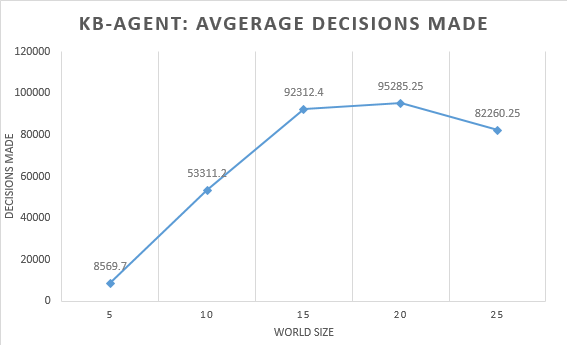
\includegraphics[width=0.8\textwidth]{figures/KBAgent_AverageDecisionsMade.PNG}
    \label{fig:KBAvgDecisions}
\end{figure}

\begin{figure}[!htb]
\caption{}
    \centering
	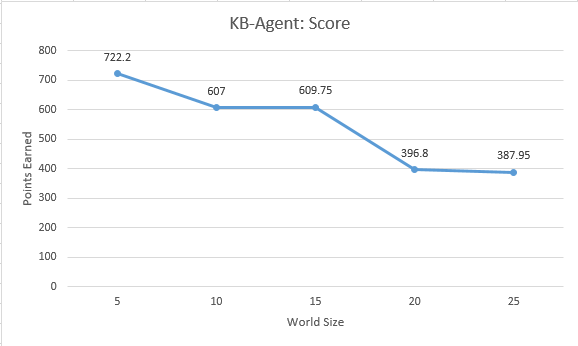
\includegraphics[width=0.8\textwidth]{figures/KBAgent_AveragePoints.PNG}
    \label{fig:KBAvgPoints}
\end{figure}

The score does decrease as world size increases.
This is likely due to a higher potential of rooms with overlapped smells and winds causing the agent to struggle to find scenarios where a room could be determined not-pit or not-Wumpus due to all adjacent rooms having smells or winds.

Also the natural result of a larger frontier will cause the agent to do a lot more path traversal and turns which lowers the points earned.

\subsection{Reactive vs. Knowledge-Based Agent Behavior} \label{subsec:RaKB-aBehavior}
An unexpected result is that both the reactive agent and the KB-Agent displayed a similar rate of change in average decisions made as the map size increased.

The fact that the inference engine keeps the KB-Agent safe from ever dying is an obvious advantage and is revealed in the difference between the average score of the two agents.
The KB-Agent also flexed its logical superiority in being able to identify and kill the Wumpi with arrows reliably.
Based on the difference in success rate and rooms explored, the ability to infer state and make decisions based off of the inference clearly made the KB-Agent the superior explorer.

\newpage
